\section{S-Parameters}
\subsection{Coaxial Filters}

\subsubsection{Task Description}
The task is to calibrate the network analyser (transmission and reflection for all 4 ports) and measure the 2-port parameters for coaxial filters
. Three specific coaxial filters were measured in this exercise: a Lowpass filter (SLP-100), a Highpass filter (SHP-100), and a Bandpass filter (SIF-70). Based on these measurements, the order of the filters and their characteristics must be determined
. Finally, the reflection coefficients are to be displayed as a Smith chart, and the transmission parameters must be displayed as logarithmic magnitude and phase
.

\vspace{0.5em}
\noindent\textit{(Note: Section 3.1.2 Schematic is excluded as the measurement involves connecting the coaxial filters directly to the network analyser, which cannot be represented by a unique standard symbol and does not require a complex circuit diagram. Section 3.1.3 Formulas and Calculations is also excluded because no derivations or manual calculation steps are required for this specific measurement.)}

\subsubsection{Measurement results}

\begin{table}[htpb]
    \centering
    \label{tab:measured_sparams}
    \begin{tabular}{|l|l|l|}
        \hline
        \textbf{Adjusted} & \textbf{Measured} & \textbf{Calculated} \\
        \hline
        \textbf{Frequency / Hz} & \textbf{S-Parameters / dB} & \textbf{Filter Type \& Characteristic} \\
        \hline
        2.025 GHz & $S_{11}$: -0.2646 dB & Lowpass Filter (SLP-100) \\
                  & $S_{21}$: -56.1171 dB & \\
                  & $S_{12}$: -53.6925 dB & \\
                  & $S_{22}$: -0.2646 dB & \\
        \hline
        2.025 GHz & $S_{11}$: -26.9644 dB & Highpass Filter (SHP-100) \\
                  & $S_{21}$: -0.2971 dB & \\
                  & $S_{12}$: -0.3061 dB & \\
                  & $S_{22}$: -26.1382 dB & \\
        \hline
        2.025 GHz & $S_{11}$: -2.0490 dB & Bandpass Filter (SIF-70) \\
                  & $S_{21}$: -13.3333 dB & \\
                  & $S_{12}$: -13.3577 dB & \\
                  & $S_{22}$: -4.1921 dB & \\
        \hline
    \end{tabular}
    \caption{Measured 2-port S-parameters for the coaxial filters at marker frequency (2.025 GHz)}
\end{table}

\subsubsection{Curves \& diagrams}

\begin{figure}[htpb]
    \centering
    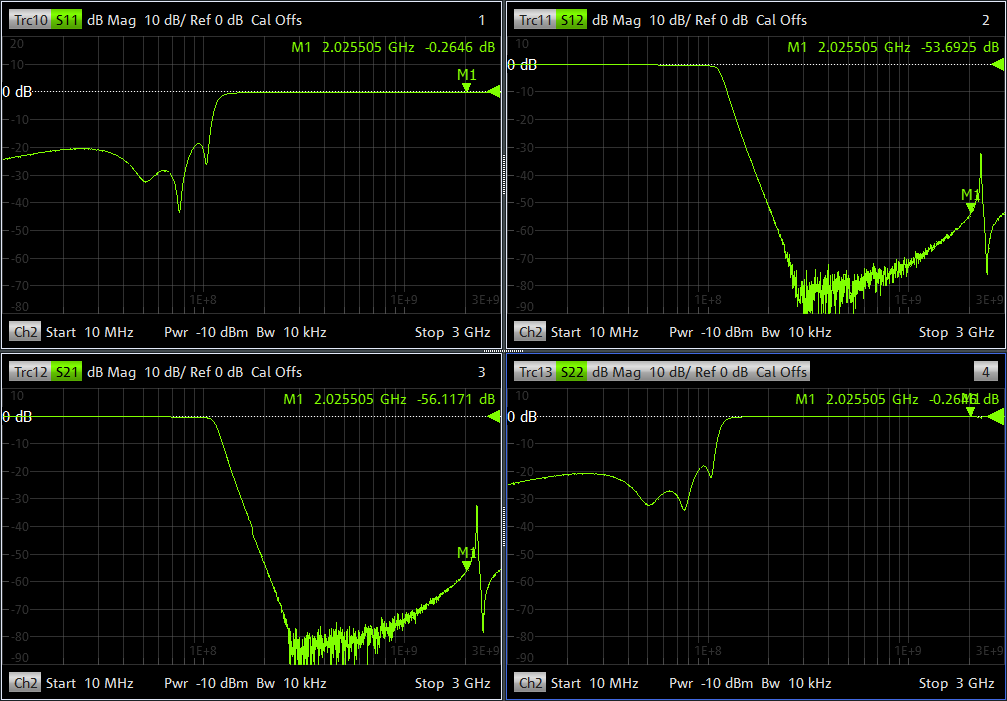
\includegraphics[width=0.8\textwidth]{src/figers/ex_3/lowpass_filter_SLP100_output_results.png}
    \caption{Transmission and reflection parameters of the SLP-100 Lowpass filter displayed as logarithmic magnitude.}
    \label{fig:lowpass_bode}
\end{figure}

\begin{figure}[htpb]
    \centering
    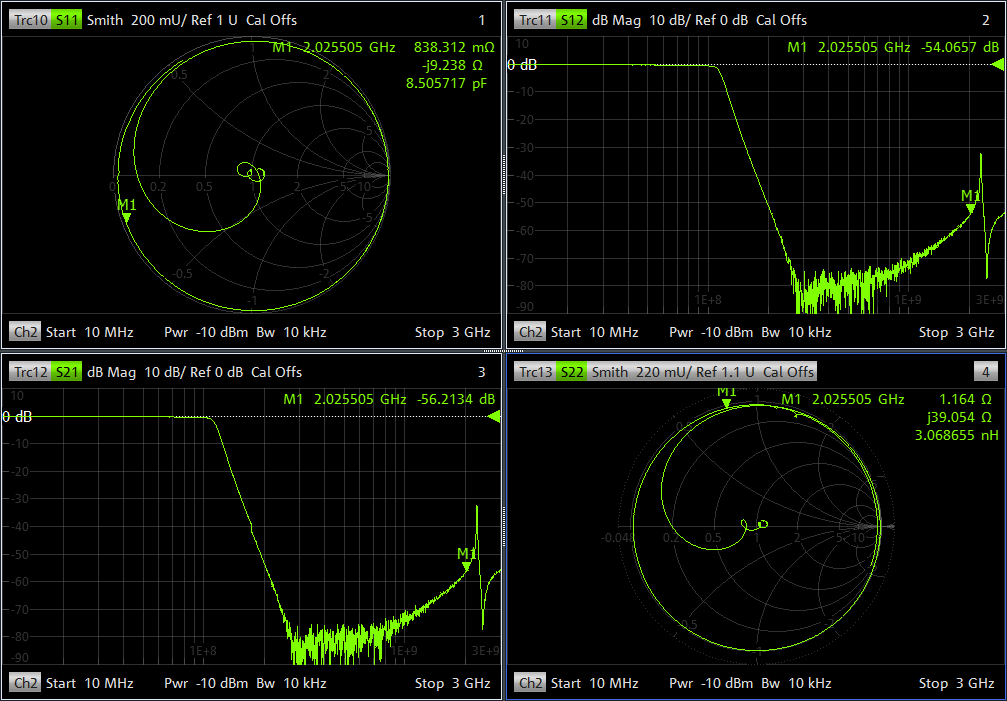
\includegraphics[width=0.8\textwidth]{src/figers/ex_3/lowpass_filter_SLP100_smith_output_results.png}
    \caption{Reflection coefficients of the SLP-100 Lowpass filter displayed in a Smith chart.}
    \label{fig:lowpass_smith}
\end{figure}

\begin{figure}[htpb]
    \centering
    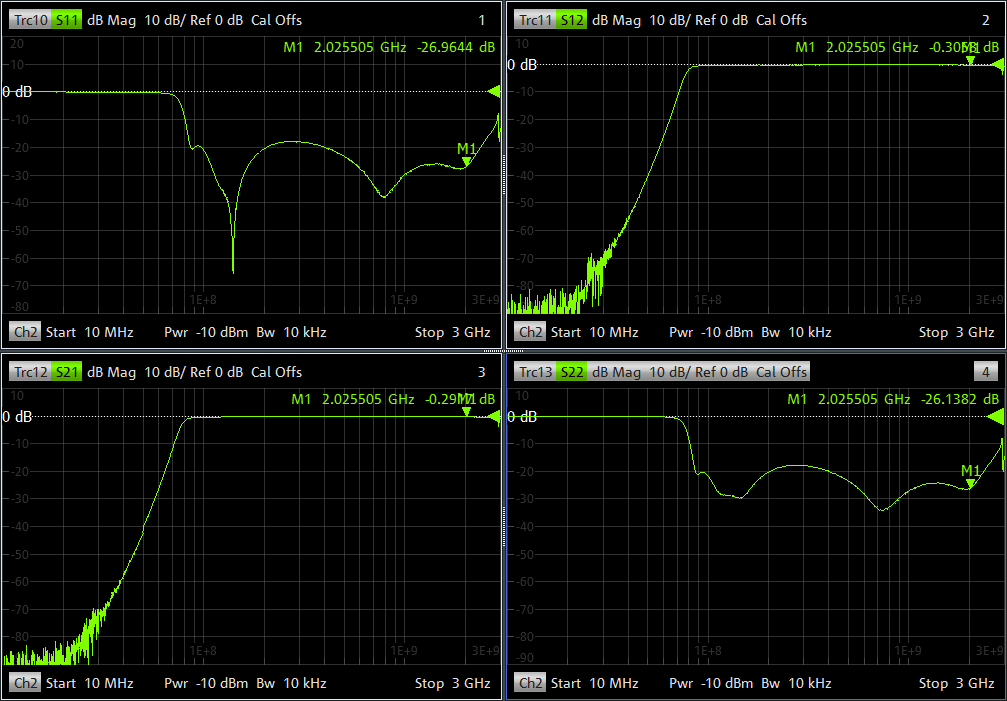
\includegraphics[width=0.8\textwidth]{src/figers/ex_3/highpass_filter_SHP100_output_results.png}
    \caption{Transmission and reflection parameters of the SHP-100 Highpass filter displayed as logarithmic magnitude.}
    \label{fig:highpass_bode}
\end{figure}

\begin{figure}[htpb]
    \centering
    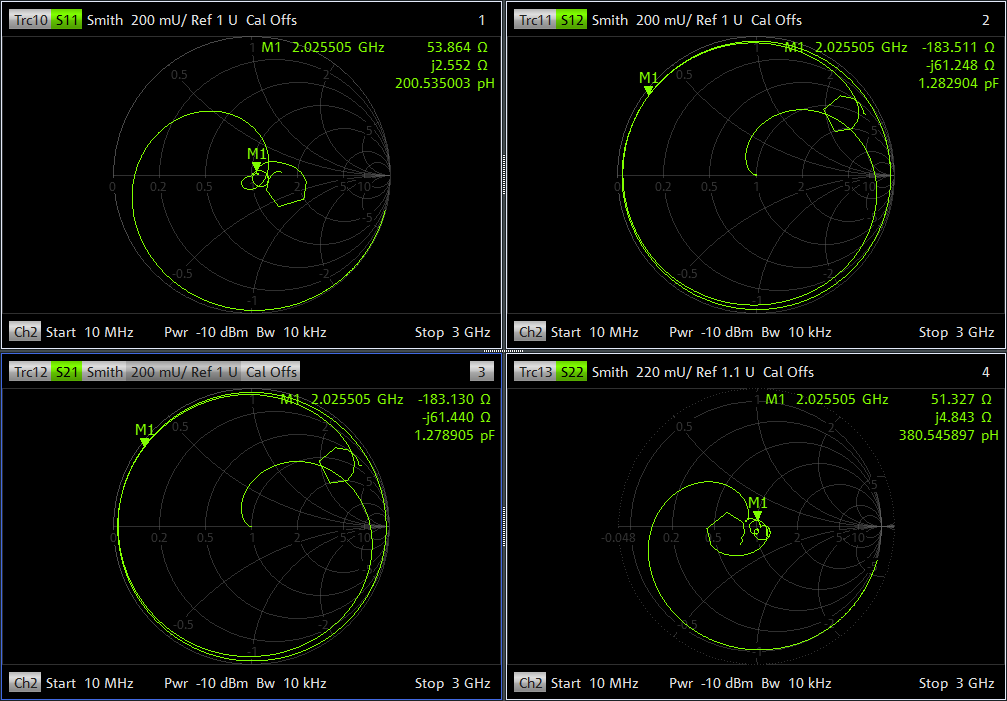
\includegraphics[width=0.8\textwidth]{src/figers/ex_3/highpass_filter_SHP100_smith_output_results.png}
    \caption{Reflection coefficients of the SHP-100 Highpass filter displayed in a Smith chart.}
    \label{fig:highpass_smith}
\end{figure}

\begin{figure}[htpb]
    \centering
    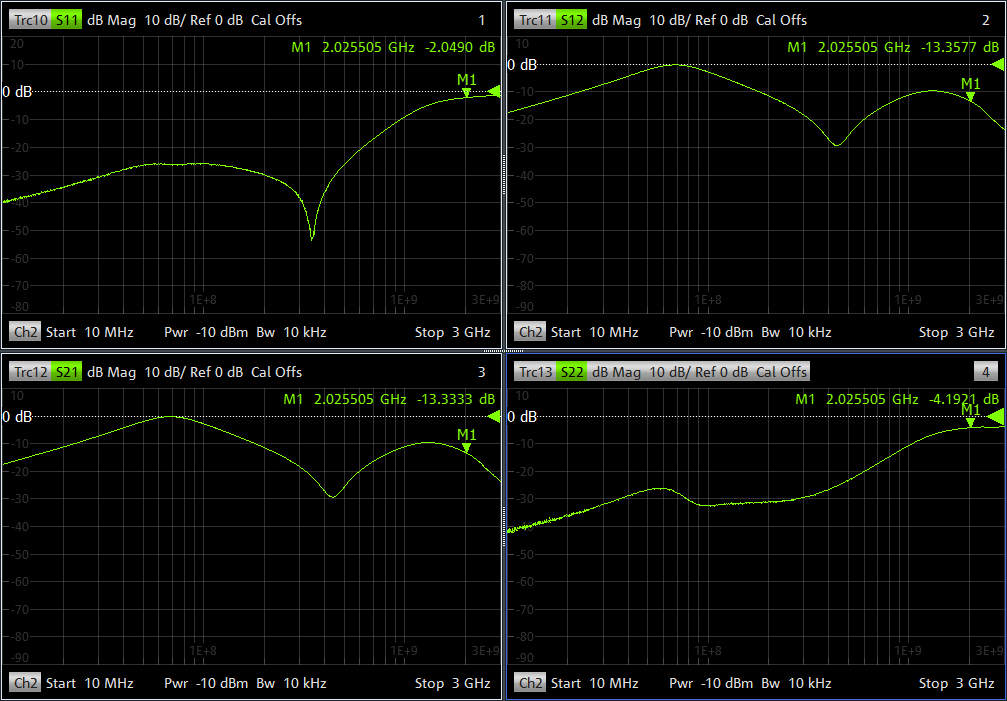
\includegraphics[width=0.8\textwidth]{src/figers/ex_3/bandpass_filter_SIF70_output_results.png}
    \caption{Transmission and reflection parameters of the SIF-70 Bandpass filter displayed as logarithmic magnitude.}
    \label{fig:bandpass_bode}
\end{figure}

\begin{figure}[htpb]
    \centering
    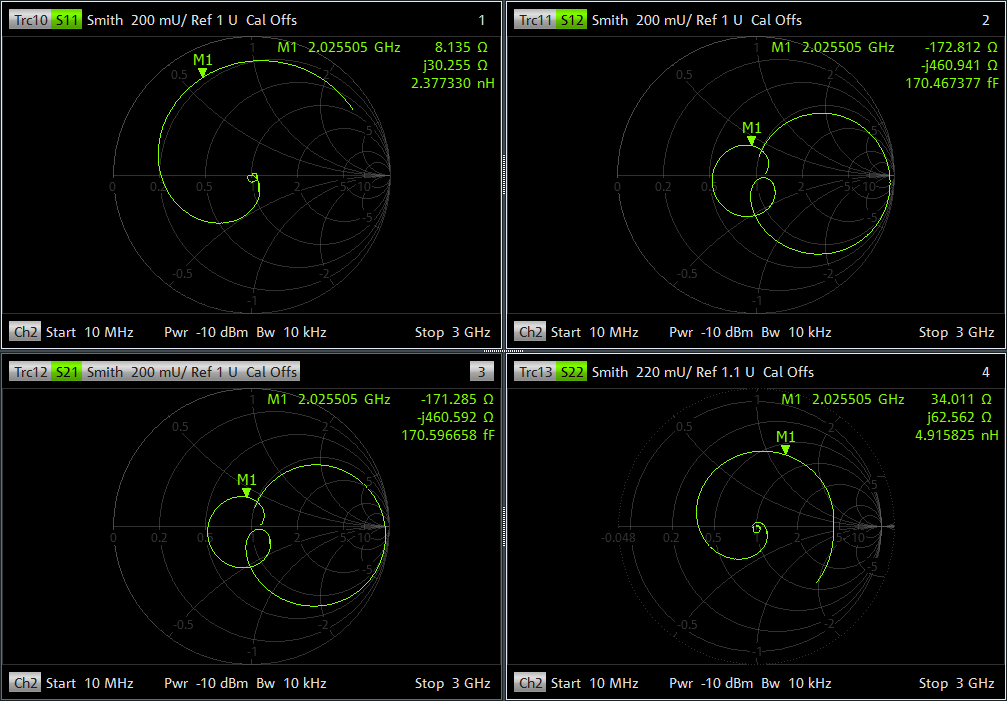
\includegraphics[width=0.8\textwidth]{src/figers/ex_3/bandpass_filter_SIF70_smith_output_results.png}
    \caption{Reflection coefficients of the SIF-70 Bandpass filter displayed in a Smith chart.}
    \label{fig:bandpass_smith}
\end{figure}

\FloatBarrier

\subsubsection{Short discussion of measurement results}

Considering the measured transmission and reflection parameters, the distinct characteristics of the three filters can be clearly identified:

\begin{itemize}
    \item \textbf{Lowpass Filter (SLP-100):} The magnitude plot exhibits a clear low-pass characteristic, passing frequencies below approximately 100 MHz. In the stopband at the 2.025 GHz marker, the transmission ($S_{21}$) is highly attenuated (-56.11 dB), while the reflection ($S_{11}$) is nearly 0 dB (-0.26 dB). This indicates that in the stopband, the rejected signal is almost entirely reflected rather than absorbed. The Smith chart confirms this, as the impedance trace moves tightly along the highly reactive outer boundary for stopband frequencies.
    
    \item \textbf{Highpass Filter (SHP-100):} This filter demonstrates a high-pass response, heavily attenuating low frequencies but allowing frequencies above $\sim$100 MHz to pass. At the 2.025 GHz marker (which falls within the passband), the transmission is excellent with negligible insertion loss ($S_{21}$ = -0.29 dB) and the reflection is minimized ($S_{11}$ = -26.96 dB). On the Smith chart, the passband frequencies converge securely near the 50 $\Omega$ center matching point.
    
    \item \textbf{Bandpass Filter (SIF-70):} The magnitude plot reveals a distinct passband centered near 70 MHz. At higher frequencies outside this band, such as the 2.025 GHz marker, the signal transmission is attenuated ($S_{21}$ = -13.33 dB) and the reflection increases accordingly ($S_{11}$ = -2.04 dB).
\end{itemize}

Regarding the order of the filters, it can be estimated by observing the attenuation slope in the stopband of the logarithmic magnitude plots. The extreme steepness of the transition from the passband to the stopband - particularly visible as a sharp, near-vertical drop in the SLP-100 and SHP-100 plots—indicates a high roll-off rate per decade. This suggests that these components are higher-order filters, which is necessary to provide such a rapid cut-off.

\subsection{Microstrip Lines}

\subsubsection{Task Description}
The task is to measure the transmission coefficient ($S_{21}$) and the reflection coefficient ($S_{11}$) for different microstrip lines using a network analyser. Based on the measurement data obtained, this section focuses on a comparative analysis of the reflection coefficients ($S_{11}$) of five distinct microstrip configurations, utilizing the instrument's memory traces to display them simultaneously.

\subsubsection{Schematic}
\textit{(Placeholder: Insert your "Figure 3.1: Measured Microstrip-Lines" photograph here. As per the guidelines, the network analyser itself does not need to be drawn in detail, but the measuring points connecting to the microstrip lines must be clearly indicated.)}

\vspace{0.5em}
\noindent\textit{(Note: Section 3.2.3 Formulas and Calculations is excluded as the task relies on direct network analyser measurements, and no specific analytical derivations are required to present the $S_{11}$ data.)}

\subsubsection{Table(s) with measurement results}

The Voltage Standing Wave Ratio (VSWR) is calculated from the measured $S_{11}$ magnitude in decibels using the formula:
\begin{equation}
    \text{VSWR} = \frac{1 + 10^{(S_{11}/20)}}{1 - 10^{(S_{11}/20)}}
\end{equation}

\begin{table}[htpb]
    \centering
    \label{tab:microstrip_vswr}
    \begin{tabular}{|l|l|l|}
        \hline
        \textbf{Adjusted} & \textbf{Measured} & \textbf{Calculated} \\
        \hline
        \textbf{Frequency / Hz} & \textbf{$S_{11}$ / dB} & \textbf{VSWR} \\
        \hline
        2.025 GHz & Line 1 (Green Trace): -24.2573 dB & 1.13 \\
        \hline
        2.025 GHz & Line 2 (Cyan Trace): -16.9885 dB & 1.33 \\
        \hline
        2.025 GHz & Line 3 (Orange Trace): -23.9754 dB & 1.13 \\
        \hline
        2.025 GHz & Line 4 (Red Trace): -14.3692 dB & 1.47 \\
        \hline
        2.025 GHz & Line 5 (Yellow Trace): -20.9835 dB & 1.20 \\
        \hline
    \end{tabular}
    \caption{Measured reflection coefficients and calculated VSWR for the microstrip lines at marker M1 (2.025 GHz)}
\end{table}

\subsubsection{Curves \& diagrams}

\begin{figure}[htpb]
    \centering
    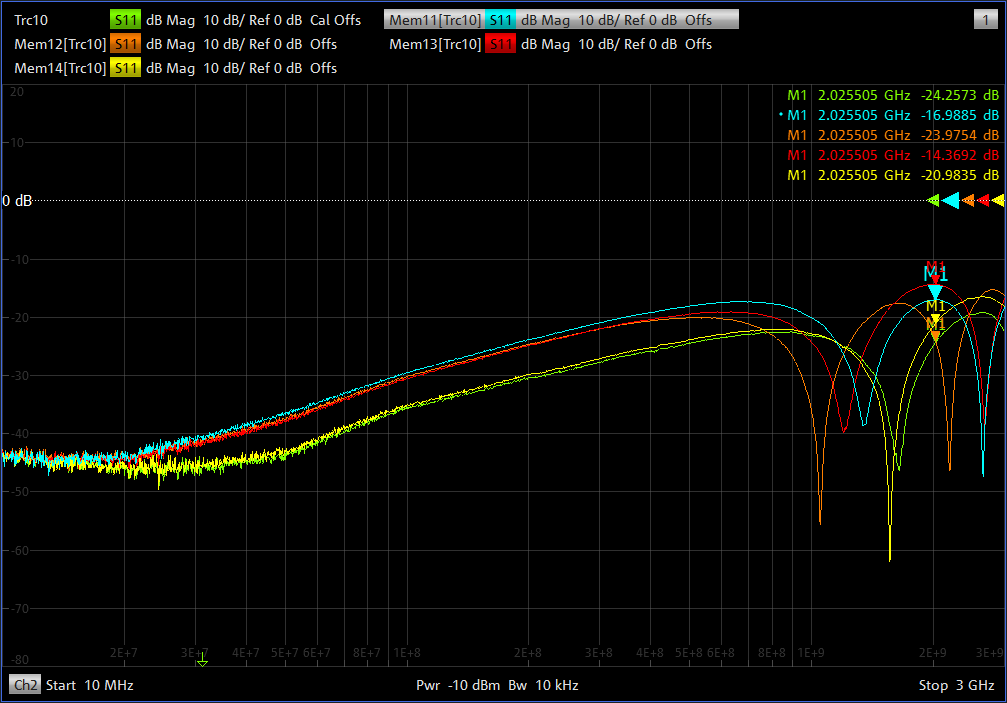
\includegraphics[width=0.8\textwidth]{src/figers/ex_3/C5_microstrip_output.png}
    \caption{Measured reflection coefficients ($S_{11}$) of five different microstrip lines over a 3 GHz span, compared using memory traces.}
    \label{fig:microstrip_comparison}
\end{figure}

\begin{figure}[htpb]
    \centering
    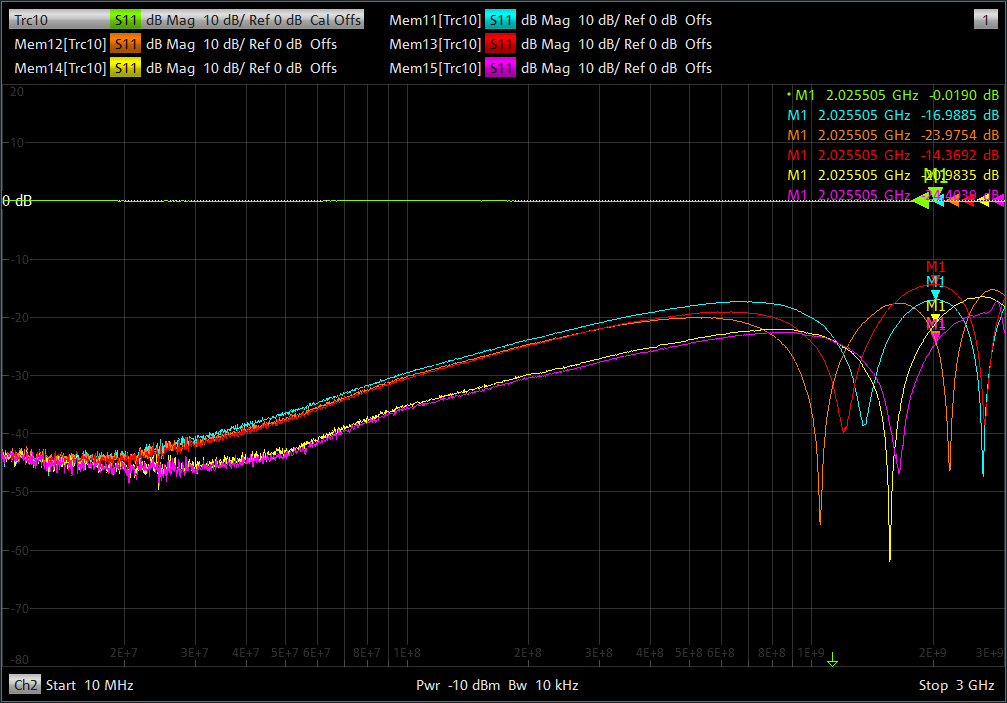
\includegraphics[width=0.8\textwidth]{src/figers/ex_3/C5_disconnected_microstrip_output.png}
    \caption{Reflection coefficient comparison including a disconnected microstrip line (Green Trace, M1 = -0.0318 dB), demonstrating total reflection.}
    \label{fig:microstrip_disconnected}
\end{figure}
\FloatBarrier

\subsubsection{Short discussion of measurement results}

Based on the plotted diagrams, one can observe the distinct reflection coefficient ($S_{11}$) envelopes for all the measured microstrip lines. At very low frequencies (starting at 10 MHz), the reflection coefficients are extremely low (approximately -45 dB), indicating excellent impedance matching to the 50 $\Omega$ system. As the frequency increases towards 3 GHz, the overall envelope of the reflection coefficients degrades (rising to approximately -15 dB). This progressive mismatch is a result of the frequency-dependent dielectric losses, conductor losses, and parasitic reactances inherent to the microstrip structures and their SMA connector transitions.

As clearly visible in the plots, every reflection coefficient curve exhibits periodic, sharp minima (approximately four deep minima across the 3 GHz spectrum). At every minimum, the reflection coefficient drops significantly toward 0, which means that at these specific resonant frequencies, the given microstrip line is exceptionally well-matched and presents an input impedance of almost exactly 50 $\Omega$.

Furthermore, Figure 3-8 includes a measurement of a disconnected microstrip line (represented by the flat green trace). Because the line is open-ended, the boundary condition creates an infinite load impedance, resulting in a theoretical reflection factor of $\rho = +1$. This is perfectly validated by the measurement, which shows a constant $S_{11}$ magnitude of approximately 0 dB (-0.0190 dB at 2.025 GHz) across the entire frequency range, confirming that the signal is being entirely reflected back to the source.

\subsection{3-Port Circulator}

\subsubsection{Task Description}
The objective of this task is to measure the complete S-parameter matrix of a 3-port circulator using a network analyser and compare the measured characteristics against the ideal theoretical behaviour of a circulator. Two different physical components were measured: a larger circulator optimized for the $\sim$900 MHz band, and a smaller circulator optimized for the $\sim$2.4 GHz band.

\subsubsection{Schematic}
\textit{(Placeholder: Insert the block diagram or standard symbol of the 3-port circulator here with its ports clearly labeled 1, 2, and 3. As per the guidelines, the network analyser itself does not need to be drawn, but the measuring points connecting to the circulator ports must be marked clearly.)}

\subsubsection{Formulas and Calculations}
A circulator is an asymmetric, non-reciprocal component. According to the laboratory manual, the ideal scattering matrix (S-matrix) of a perfectly matched, lossless 3-port circulator is defined as:

\begin{equation}
    S_{\text{ideal}} = \begin{bmatrix}
    0 & 1 & 0 \\
    0 & 0 & 1 \\
    1 & 0 & 0
    \end{bmatrix}
\end{equation}

Network analysers display the measured transmission and reflection coefficients in decibels (dB). To directly compare the measured results with the ideal linear voltage ratios shown in the theoretical matrix, the measured dB values must be converted back to linear magnitudes using the calculation: 

\begin{equation}
    |S_{\text{linear}}| = 10^{\frac{S_{\text{dB}}}{20}}
\end{equation}

\subsubsection{Table(s) with measurement results}

\begin{table}[htpb]
    \centering
    \label{tab:circulator_results}
    \begin{tabular}{|l|l|l|}
        \hline
        \textbf{Adjusted} & \textbf{Measured} & \textbf{Calculated} \\
        \hline
        \textbf{Frequency / Hz} & \textbf{S-Parameters / dB} & \textbf{Linear Magnitude $|S_{\text{linear}}|$} \\
        \hline
        901.327 MHz & Bigger Circulator (Forward Transmission) & \\
                    & $S_{21}$: -0.1956 dB & $|S_{21}|$: 0.9777 \\
                    & $S_{32}$: -0.1992 dB & $|S_{32}|$: 0.9773 \\
                    & $S_{13}$: -0.1919 dB & $|S_{13}|$ : 0.9781 \\
        \hline
        901.327 MHz & Bigger Circulator (Reflection \& Isolation) & \\
                    & $S_{11}$: -35.9381 dB, $S_{22}$: -32.7119 dB, $S_{33}$: -38.2485 dB & $|S_{11}|$: 0.0160, $|S_{22}|$: 0.0231, $|S_{33}|$: 0.0122 \\
                    & $S_{12}$: -32.7563 dB, $S_{23}$: -33.7612 dB, $S_{31}$: -30.5914 dB & $|S_{12}|$: 0.0230, $|S_{23}|$: 0.0205, $|S_{31}|$: 0.0295 \\
        \hline
        2.436 GHz   & Small Circulator (Forward Transmission) & \\
                    & $S_{21}$: -0.1491 dB & $|S_{21}|$: 0.9830 \\
                    & $S_{32}$: -0.1557 dB & $|S_{32}|$: 0.9822 \\
                    & $S_{13}$: -0.1704 dB & $|S_{13}|$: 0.9806 \\
        \hline
        2.436 GHz   & Small Circulator (Reflection \& Isolation) & \\
                    & $S_{11}$: -46.7460 dB, $S_{22}$: -36.3968 dB, $S_{33}$: -31.3121 dB & $|S_{11}|$: 0.0046, $|S_{22}|$: 0.0151, $|S_{33}|$: 0.0272 \\
                    & $S_{12}$: -37.0203 dB, $S_{23}$: -40.5446 dB, $S_{31}$: -35.8733 dB & $|S_{12}|$: 0.0141, $|S_{23}|$: 0.0094, $|S_{31}|$: 0.0161 \\
        \hline
    \end{tabular}
    \caption{Measured S-parameters and calculated linear magnitudes for the two circulators at their optimal frequencies}
\end{table}

\subsubsection{Curves \& diagrams}

\begin{figure}[htpb]
    \centering
    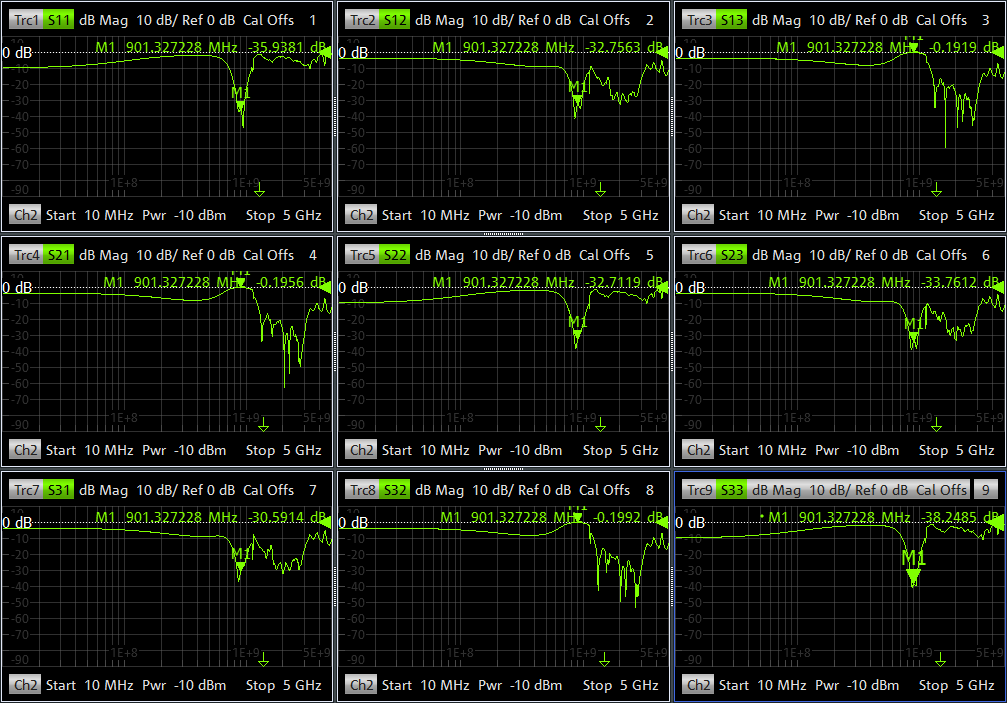
\includegraphics[width=0.8\textwidth]{src/figers/ex_3/Bigger_circ_lowfreq2.png}
    \caption{Measured S-parameter matrix of the bigger circulator with the marker set to its optimum frequency of 901.3 MHz.}
    \label{fig:bigger_circ_matrix}
\end{figure}

\begin{figure}[htpb]
    \centering
    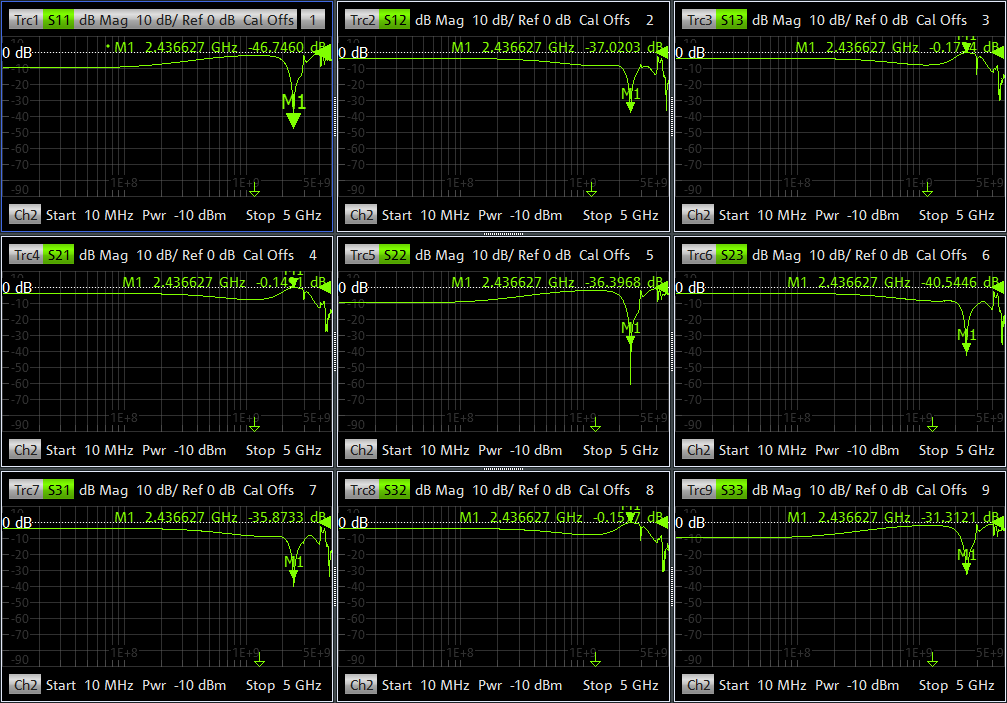
\includegraphics[width=0.8\textwidth]{src/figers/ex_3/Small_circ_lowfreq.png}
    \caption{Measured S-parameter matrix of the small circulator with the marker set to its optimum frequency of 2.436 GHz.}
    \label{fig:small_circ_matrix}
\end{figure}

\FloatBarrier

\subsubsection{Short discussion of measurement results}

By compiling the calculated linear magnitudes from Table 3.3, we can reconstruct the actual linear S-matrices for both components at their respective operating frequencies. For the 901 MHz circulator, the matrix is:

\begin{equation}
    S_{\text{901MHz}} = \begin{bmatrix}
    0.0160 & 0.0230 & 0.9781 \\
    0.9777 & 0.0231 & 0.0205 \\
    0.0295 & 0.9773 & 0.0122
    \end{bmatrix}
\end{equation}

Comparing this against the ideal theoretical matrix defined in Section 3.3.3, the characteristic behaviour of the circulator is distinctly proven. The main diagonal entries ($S_{11}$, $S_{22}$, $S_{33}$) are extremely close to 0 (all under 0.025 linear, representing excellent impedance matching and return losses better than -32 dB).

The off-diagonal elements demonstrate the non-reciprocal circular flow of power. The parameters $S_{21}$, $S_{32}$, and $S_{13}$ are all approximately 0.98. This dictates that power strictly flows in a clockwise circle: from port 1 to port 2, port 2 to port 3, and port 3 to port 1. In the reverse direction (e.g., $S_{12}$, $S_{23}$, $S_{31}$), the signal is highly isolated, with values near 0.02 (isolations exceeding 30 dB).

The matrices do not perfectly equal "1" in the forward direction because the circulator is a real, physical component subject to insertion loss. The forward paths suffer approximately 0.15 to 0.20 dB of attenuation due to ohmic losses in the conductors and magnetic losses within the ferrite material.

Finally, the measurements highlight the strict frequency dependency of circulators, which is tied to the physical size of their ferrite core. The larger circulator provides optimum matching at a longer wavelength (901 MHz), whereas the smaller circulator is required for the shorter wavelength of the 2.436 GHz frequency.

\subsection{3-Port Resistive Power Divider}

\subsubsection{Task Description}
The task is to measure the S-parameters of a 3-port resistive power divider using a network analyser. The objective is to verify that the power divider matches all three ports to the characteristic impedance and exhibits a total loss of 6 dB. Furthermore, the measurement should determine whether there is any isolation between output ports 2 and 3.

\subsubsection{Schematic}
\textit{(Placeholder: Insert the circuit diagram or block symbol of the 3-port resistive power divider here. Ensure the three ports are clearly marked as Port 1, Port 2, and Port 3. As per the guidelines, measuring points must be clearly marked.)}

\subsubsection{Formulas and Calculations}
A completely matched, reciprocal 3-port network cannot be lossless. A resistive power divider uses resistors to match all three ports simultaneously to the characteristic impedance ($Z_0$). Because of the reciprocal and symmetrical nature of this specific resistive network, the theoretical linear S-parameter matrix is expected to be:

\begin{equation}
    S = 0.5 \times \begin{bmatrix}
    0 & 1 & 1 \\
    1 & 0 & 1 \\
    1 & 1 & 0
    \end{bmatrix}
\end{equation}

Network analysers display these values in decibels (dB). The theoretical transmission loss of 0.5 corresponds to:
\begin{equation}
    S_{\text{dB}} = 20 \cdot \log(0.5) \approx -6\text{ dB}
\end{equation}
This explains the theoretical 6 dB total loss between the input and any output port.

To directly compare the measured decibel results with the ideal linear voltage ratios, the measured dB values must be converted back to linear magnitudes using the calculation: 
\begin{equation}
    |S_{\text{linear}}| = 10^{\frac{S_{\text{dB}}}{20}}
\end{equation}

\subsubsection{Table(s) with measurement results}

\begin{table}[htpb]
    \centering
    \label{tab:power_divider_results}
    \begin{tabular}{|l|l|l|}
        \hline
        \textbf{Adjusted} & \textbf{Measured} & \textbf{Calculated} \\
        \hline
        \textbf{Frequency / Hz} & \textbf{S-Parameters / dB} & \textbf{Linear Magnitude $|S_{\text{linear}}|$} \\
        \hline
        2.109886 GHz & Reflection Coefficients & \\
                     & $S_{11}$: -33.2039 dB & $|S_{11}|$ : 0.0219 \\
                     & $S_{22}$: -36.1822 dB & $|S_{22}|$: 0.0155 \\
                     & $S_{33}$: -37.5277 dB & $|S_{33}|$: 0.0133 \\
        \hline
        2.109886 GHz & Transmission Coefficients & \\
                     & $S_{21}$: -6.0411 dB, $S_{12}$: -6.0452 dB & $|S_{21}|$: 0.4988, $|S_{12}|$: 0.4986 \\
                     & $S_{31}$: -6.0823 dB, $S_{13}$: -6.0846 dB & $|S_{31}|$: 0.4965, $|S_{13}|$: 0.4963 \\
        \hline
        2.109886 GHz & Isolation Coefficients & \\
                     & $S_{23}$: -6.0447 dB, $S_{32}$: -6.0488 dB & $|S_{23}|$: 0.4986, $|S_{32}|$: 0.4984 \\
        \hline
    \end{tabular}
    \caption{Measured S-parameters of the 3-port resistive power divider at marker frequency (2.109 GHz)}
\end{table}
\FloatBarrier

\subsubsection{Curves \& diagrams}

\begin{figure}[htpb]
    \centering
    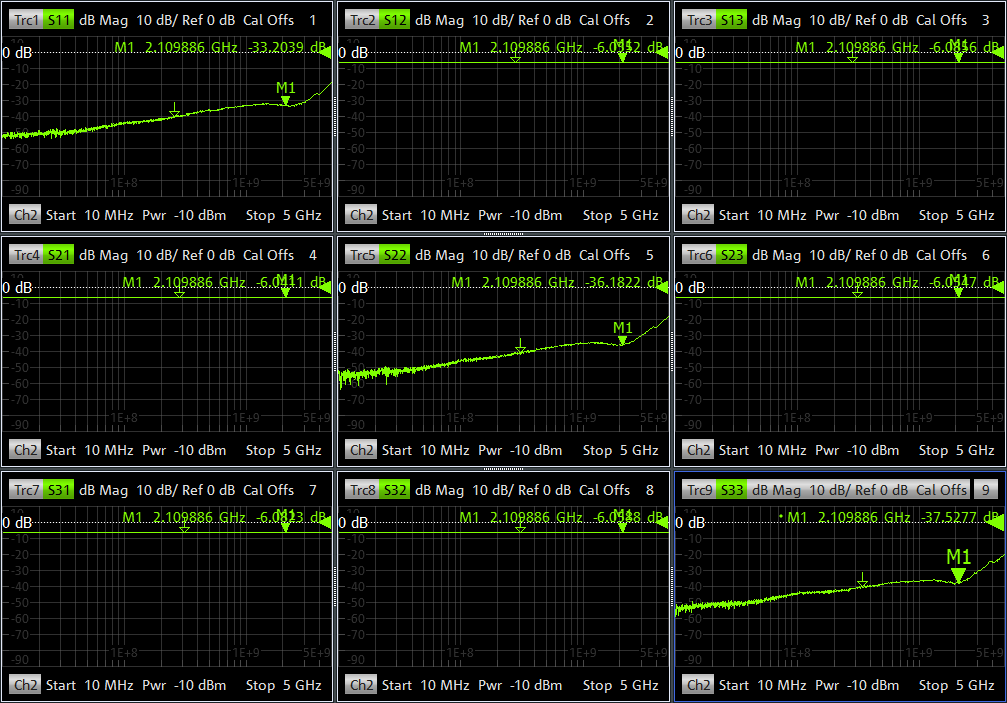
\includegraphics[width=0.8\textwidth]{src/figers/ex_3/Resistive_dividers.png}
    \caption{Measured S-parameters (transmission, reflection, and isolation) of the 3-port resistive power divider displayed as logarithmic magnitude.}
    \label{fig:resistive_dividers_bode}
\end{figure}

\begin{figure}[htpb]
    \centering
    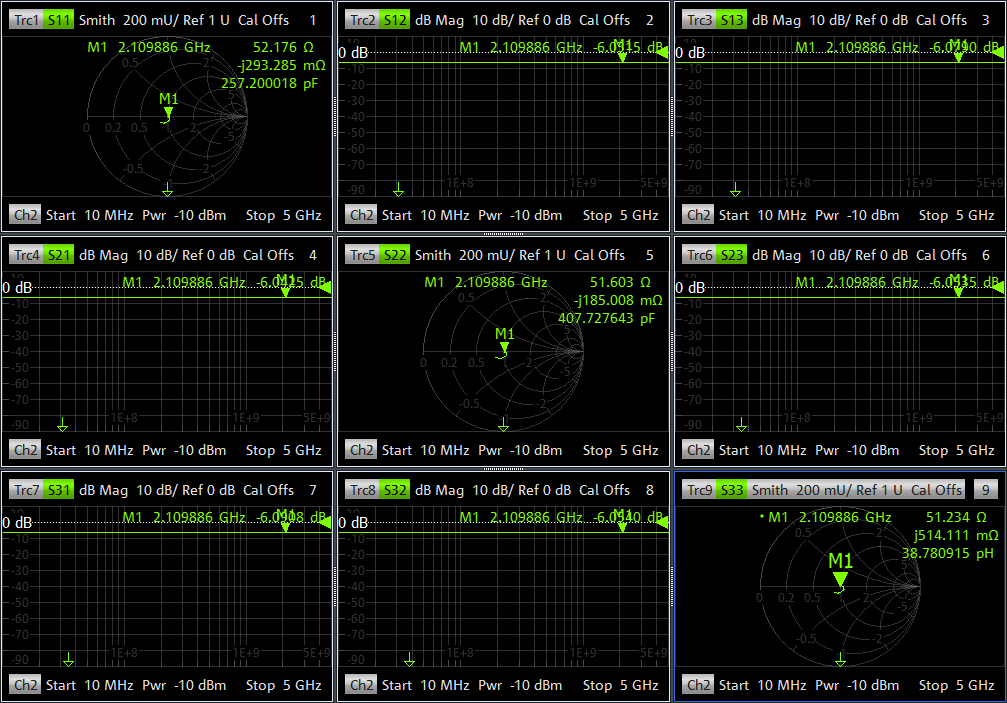
\includegraphics[width=0.8\textwidth]{src/figers/ex_3/Resistive_dividers_smith.png}
    \caption{Reflection parameters ($S_{11}$, $S_{22}$, $S_{33}$) and transmission parameters of the 3-port resistive power divider displayed in a Smith chart.}
    \label{fig:resistive_dividers_smith}
\end{figure}

\FloatBarrier

\subsubsection{Short discussion of measurement results}

Based on the measurement results, the reflection coefficients ($S_{11}$, $S_{22}$, $S_{33}$) are all below -33 dB (equivalent to a linear magnitude of less than 0.022). This confirms that all three ports are exceptionally well-matched to the 50 $\Omega$ characteristic impedance. The Smith chart perfectly validates this, as the traces for $S_{11}$, $S_{22}$, and $S_{33}$ are contracted securely into the center matching point (e.g., $S_{11}$ reads 52.17 $\Omega$ - j0.29 $\Omega$).

The forward and reverse transmission coefficients between the input and outputs ($S_{21}$, $S_{12}$, $S_{31}$, $S_{13}$) were measured at approximately -6.04 dB to -6.08 dB. Converting these values yields a linear voltage ratio of approximately 0.498. This practically confirms the theoretical total loss of 6 dB inherent to a resistive 3-port matching network.

Regarding the relationship between ports 2 and 3, the measured parameters $S_{23}$ and $S_{32}$ are approximately -6.04 dB. This explicitly demonstrates that there is no isolation between port 2 and port 3. The signal is freely transmitted between these two output ports, experiencing the exact same 6 dB attenuation as the main input-to-output path. This lack of isolation is the defining difference between a basic resistive power divider and a Wilkinson power divider (which provides high isolation between its outputs). The slight deviations of roughly 0.04 to 0.08 dB from the ideal 6 dB value can be attributed to the component tolerances of the internal resistors and minor parasitic effects at 2.1 GHz.

\subsection{Antenna Reflection Coefficients}

\subsubsection{Task Description}
The task is to measure the reflection coefficient ($S_{11}$) of different antennas using a network analyser. Based on the measurements, the reflection characteristics of two different antenna configurations (Antenna 1 and Antenna 2 with a ground plane) are evaluated. The measurement results must be displayed both as a Smith chart and as a logarithmic magnitude plot over frequency.

\subsubsection{Schematic}
\textit{(Placeholder: As the measurement involves connecting the antennas directly to the network analyser’s port, a full circuit diagram is not strictly necessary. If you have photographs of the physical antennas or the measurement setup, insert them here.)}

\subsubsection{Formulas and Calculations}
The reflection factor $\rho$ (which corresponds to the $S_{11}$ parameter measured by the network analyser) at the point of the load is defined as the ratio of the backward to the forward voltage wave. It relates the antenna’s input impedance ($Z_L$) to the characteristic impedance of the measurement system ($Z_w$, typically 50 $\Omega$):

\begin{equation}
    \rho = \frac{Z_L - Z_w}{Z_L + Z_w}
\end{equation}

The network analyser displays the logarithmic magnitude of the reflection coefficient in decibels, calculated as:

\begin{equation}
    S_{11[\text{dB}]} = 20 \cdot \log(|S_{11}|)
\end{equation}

To assess the matching quality, the Voltage Standing Wave Ratio (VSWR) is calculated from the linear reflection magnitude $|S_{11}|$:

\begin{equation}
    \text{VSWR} = \frac{1 + |S_{11}|}{1 - |S_{11}|}
\end{equation}

\subsubsection{Table(s) with measurement results}

\begin{table}[htpb]
    \centering
    \label{tab:antenna_results}
    \begin{tabular}{|l|l|l|}
        \hline
        \textbf{Adjusted} & \textbf{Measured} & \textbf{Calculated} \\
        \hline
        \textbf{Frequency / Hz} & \textbf{Reflection Coefficient $S_{11}$ / dB} & \textbf{Impedance $Z_L$ / $\Omega$ and VSWR} \\
        \hline
        3.049430 GHz & Antenna 1 (Corrected) & \\
                     & $S_{11}$: -9.6100 dB & $Z_L$: 38.34 $\Omega$ - j28.07 $\Omega$ \\
                     & & VSWR: 1.99 \\
        \hline
        2.512917 GHz & Antenna 2 (with Ground Plane) & \\
                     & $S_{11}$: -27.2397 dB & $Z_L$: 47.76 $\Omega$ + j3.44 $\Omega$ (at 2.525 GHz) \\
                     & & VSWR: 1.09 \\
        \hline
    \end{tabular}
    \caption{Measured reflection coefficients and calculated VSWR at the resonance frequencies of the antennas}
\end{table}

\subsubsection{Curves \& diagrams}

\begin{figure}[htpb]
    \centering
    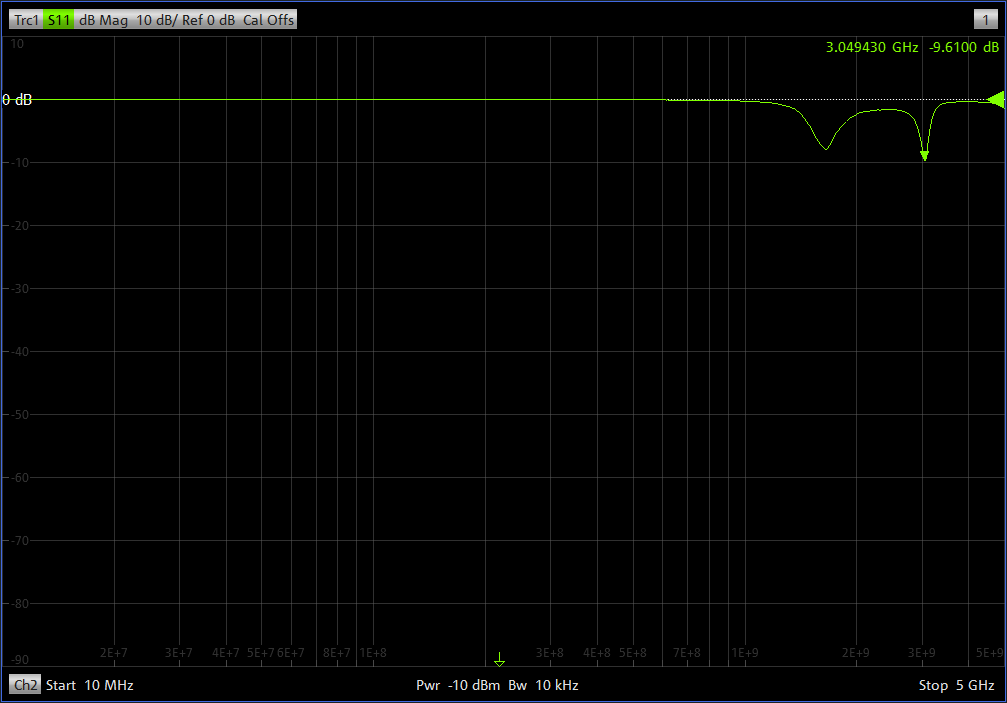
\includegraphics[width=0.8\textwidth]{src/figers/ex_3/Antenna_1_mag_CORR.png}
    \caption{Measured reflection coefficient of Antenna 1 displayed as logarithmic magnitude.}
    \label{fig:antenna1_mag}
\end{figure}

\begin{figure}[htpb]
    \centering
    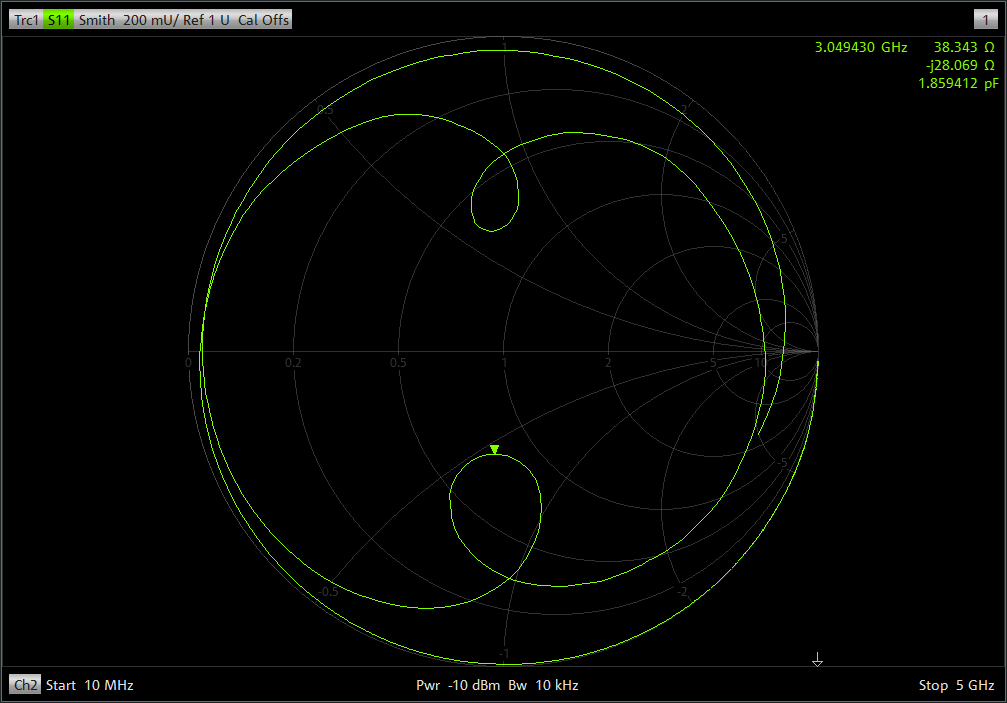
\includegraphics[width=0.8\textwidth]{src/figers/ex_3/Antenna_1_smith_CORR.png}
    \caption{Measured reflection coefficient of Antenna 1 displayed in a Smith chart.}
    \label{fig:antenna1_smith}
\end{figure}

\begin{figure}[htpb]
    \centering
    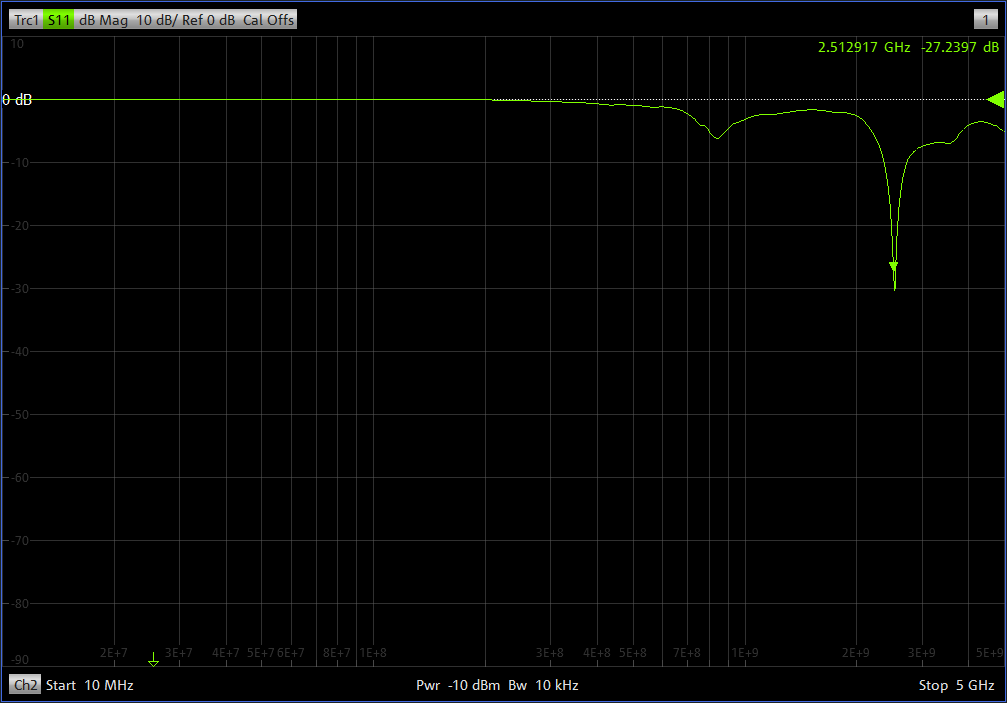
\includegraphics[width=0.8\textwidth]{src/figers/ex_3/Antenna_2_GND_CORR.png}
    \caption{Measured reflection coefficient of Antenna 2 (with ground plane) displayed as logarithmic magnitude.}
    \label{fig:antenna2_mag}
\end{figure}

\begin{figure}[htpb]
    \centering
    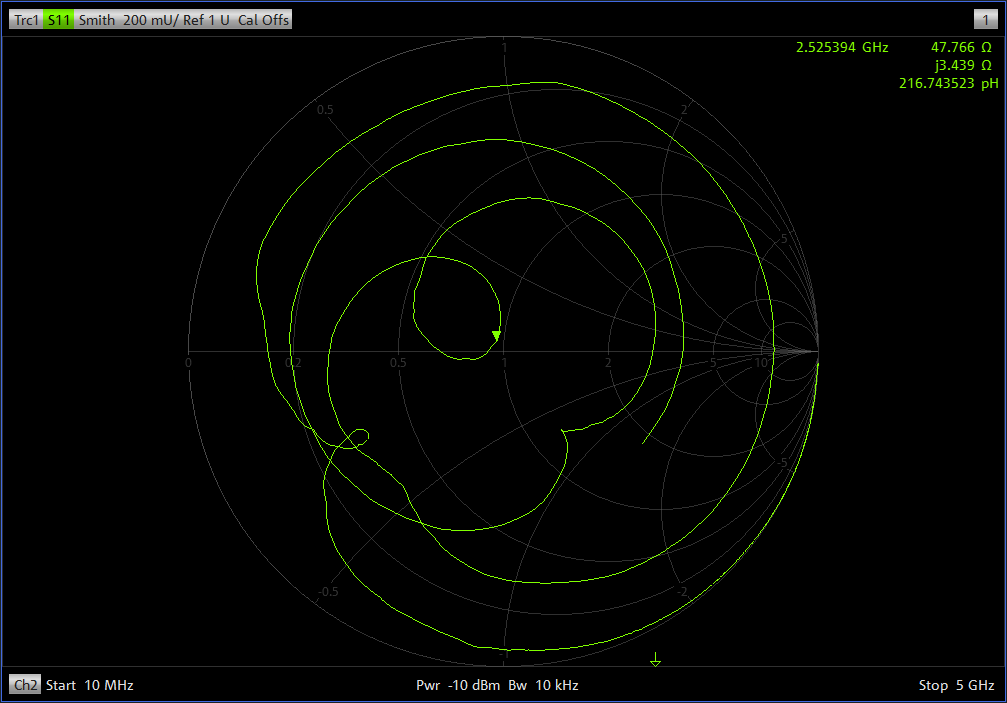
\includegraphics[width=0.8\textwidth]{src/figers/ex_3/Antenna_2_GND_smithCORR.png}
    \caption{Measured reflection coefficient of Antenna 2 (with ground plane) displayed in a Smith chart.}
    \label{fig:antenna2_smith}
\end{figure}
\FloatBarrier

\subsubsection{Short discussion of measurement results}

Based on the logarithmic magnitude plots, the distinct matching characteristics of the two antenna setups are clearly visible. Antenna 1 exhibits a moderate resonance at approximately 3.05 GHz, where the reflection coefficient reaches a minimum of -9.61 dB. Converting this value yields a VSWR of roughly 1.99. Analyzing the corresponding Smith chart confirms this slight mismatch: at 3.05 GHz, the normalised input impedance does not perfectly reach the center, presenting a slightly capacitive impedance of 38.34 $\Omega$ - j28.07 $\Omega$.

In contrast, Antenna 2 (measured with a ground plane) demonstrates excellent matching characteristics. The logarithmic magnitude plot reveals a deep, sharp resonance at 2.51 GHz with a reflection coefficient of -27.24 dB (VSWR of 1.09). By observing its Smith chart, it is evident that at resonance, the curve passes extremely close to the optimal 50 $\Omega$ matching point in the center ($r=1$, $x=0$). At the marker, the impedance reads 47.76 $\Omega$ + j3.44 $\Omega$, indicating that the reactive components have been almost entirely cancelled out, allowing for maximum power transfer from the 50 $\Omega$ system into the antenna structure.

\subsection{Unmatched Antenna and Matching Network}

\subsubsection{Task Description}
The first objective of this task is to measure the reflection coefficient (magnitude and phase) of an unmatched antenna at a given frequency. Based on this measurement, an impedance matching network consisting of a transmission line and a series capacitor must be calculated to match the antenna to the 50 $\Omega$ system. The solution must be derived using two methods: an analytical calculation and a graphical solution using the Smith chart. Finally, the calculated matching network is to be implemented (if applicable) or verified to observe the final matched reflection coefficient.

\subsubsection{Schematic}
\textit{(Placeholder: Insert two block diagrams here. The first should show the unmatched antenna connected to the network analyser port. The second should show the equivalent circuit of the matching network: the antenna $Z_A$ connected to a transmission line of length $l_e$, followed by a series capacitor $C$ connecting to the 50 $\Omega$ measurement port.)}

\subsubsection{Formulas and Calculations}

The unmatched antenna presents a load impedance $Z_A$ which can be determined from the measured reflection coefficient $\rho_A = |\rho_A| \cdot e^{j\delta}$. The normalized load impedance is $z_A = Z_A / Z_w$.

\vspace{0.5em}
\noindent\textbf{a) Analytical Solution:}\\
To match the antenna using a lossless transmission line (length $l_e$) and a series reactive element ($jX_s$), the reflection coefficient is transformed along the line towards the generator:
\begin{equation}
    \rho^+(-l_e) = \rho_A \cdot e^{-j \frac{4\pi l_e}{\lambda}}
\end{equation}

The normalized impedance at this point is $z^+(-l_e) = \frac{1 + \rho^+(-l_e)}{1 - \rho^+(-l_e)}$. Adding the series reactance $jx_s$, the total normalized impedance must equal the matching condition ($1 + j0$):
\begin{equation}
    jx_s + z^+(-l_e) - 1 = 0
\end{equation}

By separating this equation into real and imaginary parts, the two unknown quantities ($x_s$ and $l_e$) can be calculated. The normalized reactance $x_s$ is found via:
\begin{equation}
    x_s = \pm \frac{2 \cdot |\rho_A|}{\sqrt{1 - |\rho_A|^2}}
\end{equation}

Since the matching network specifically requires a capacitor, the negative solution for $x_s$ must be chosen. The actual capacitance $C$ is then calculated from the denormalized reactance $X_s = Z_w \cdot x_s$:
\begin{equation}
    X_s = -\frac{1}{\omega \cdot C} \quad \Rightarrow \quad C = -\frac{1}{\omega \cdot X_s}
\end{equation}

\vspace{0.5em}
\noindent\textbf{b) Smith Chart Solution:}\\
In the Smith chart, the initial normalized impedance $z_A$ is plotted. Moving along the transmission line corresponds to rotating clockwise (towards the generator) along the constant $|\rho_A|$ circle. The rotation stops when this circle intersects the matching circle (the $r = 1$ circle). The distance rotated along the outer wavelength scale determines the required line length $l_e$. At this intersection, the impedance has the form $1 + jx$. To achieve perfect matching, a series capacitor providing a normalized reactance of $-jx$ must be added to move the point to the centre of the Smith chart ($1 + j0$).

\subsubsection{Table(s) with measurement results}

\begin{table}[htpb]
    \centering
    \label{tab:unmatched_antenna_results}
    \begin{tabular}{|l|l|l|}
        \hline
        \textbf{Adjusted} & \textbf{Measured} & \textbf{Calculated} \\
        \hline
        \textbf{Frequency / Hz} & \textbf{Unmatched $\rho_A$ Mag / dB} & \textbf{Unmatched $Z_A$ / $\Omega$} \\
        \hline
        2.400000 GHz & $S_{11}$: -5.32 dB & $Z_A$: 113.76 $\Omega$ - j73.63 $\Omega$ \\
        \hline
        \textbf{Frequency / Hz} & \textbf{Unmatched $\rho_A$ Phase / $^\circ$} & \textbf{Required line length $l_e$ / m} \\
        \hline
        2.400000 GHz & Phase: -24.9$^\circ$ & $l_e$: 0.0483 m (4.83 cm) \\
        \hline
        \textbf{Frequency / Hz} & \textbf{Matched $S_{11}$ / dB} & \textbf{Required Capacitance $C$ / F} \\
        \hline
        2.400000 GHz & $S_{11}$: -40.42 dB & $C$: 1.03 pF \\
        \hline
    \end{tabular}
    \caption{Measurement of the unmatched antenna and calculated matching network parameters}
\end{table}
\FloatBarrier

\subsubsection{Curves \& diagrams}

\begin{figure}[htpb]
    \centering
    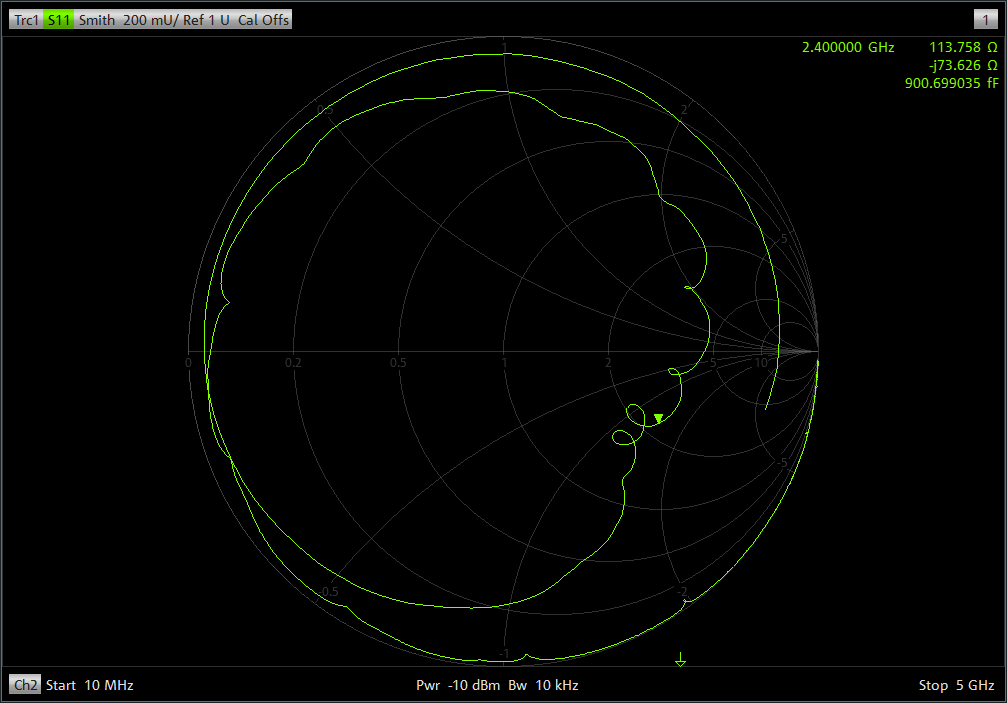
\includegraphics[width=0.8\textwidth]{src/figers/ex_3/Antenna_1_smith.png}
    \caption{Measured reflection coefficient of the unmatched antenna at 2.4 GHz displayed in a Smith chart.}
    \label{fig:unmatched_antenna_smith}
\end{figure}

\begin{figure}[htpb]
    \centering
    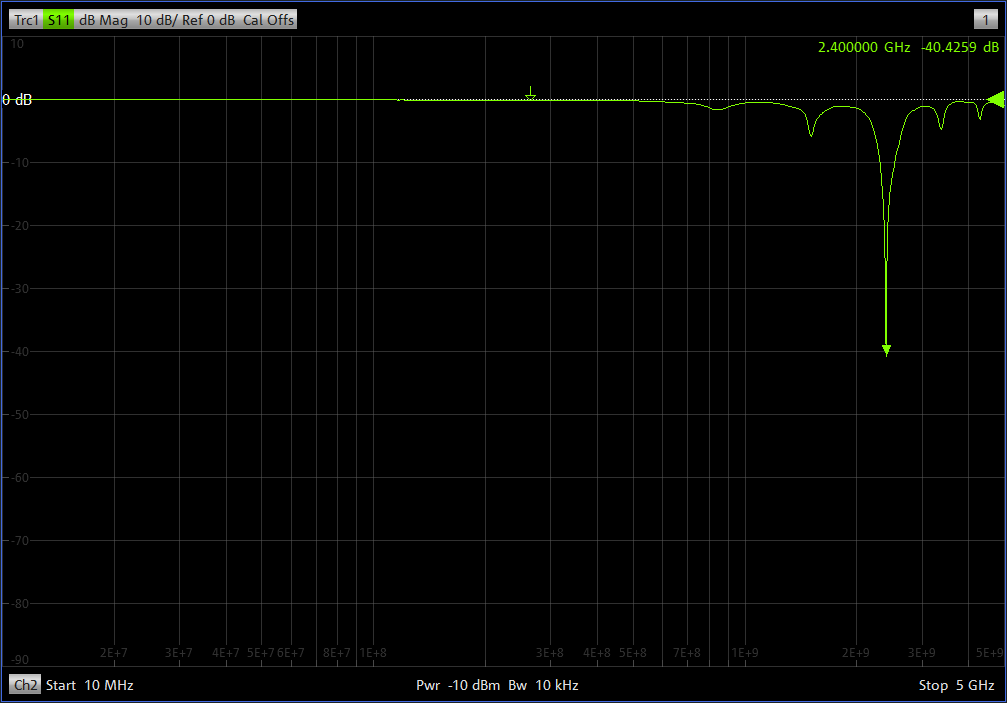
\includegraphics[width=0.8\textwidth]{src/figers/ex_3/Antenna_ss_turner_mag.png}
    \caption{Measured reflection coefficient (logarithmic magnitude) of the antenna matched to 2.4 GHz.}
    \label{fig:matched_antenna_mag}
\end{figure}
\FloatBarrier

\subsubsection{Short discussion of measurement results}

The initial measurement of the unmatched antenna at 2.4 GHz yielded an input impedance of $Z_A = 113.76\ \Omega - j73.63\ \Omega$. Converting this impedance relative to the 50 $\Omega$ system yielded a reflection coefficient magnitude of $|\rho_A| = 0.5424$ (equivalent to -5.32 dB) and a phase angle of -24.9$^\circ$. This indicates a high degree of mismatch, as more than 54\% of the voltage wave is reflected back to the source.

Using the analytical formulas, the required matching network was determined. By setting $x_s = \frac{-2 \cdot |\rho_A|}{\sqrt{1 - |\rho_A|^2}}$, a normalized series reactance of -1.291 was calculated. Denormalizing this value to 50 $\Omega$ and evaluating at 2.4 GHz resulted in a required series capacitance of $C = 1.03$ pF. The required transmission line length to rotate the reflection coefficient to this exact reactive matching point was calculated as $l_e = 4.83$ cm ($0.386\ \lambda$).

The graphical Smith chart method perfectly aligned with these calculations. By plotting the unmatched impedance and rotating clockwise along the constant $|\rho| = 0.5424$ circle, the intersection with the $r = 1$ matching circle is found exactly at the normalized impedance coordinate of $1 + j1.291$. Adding the calculated series capacitor cancels out the $+j1.291$ reactance, pulling the impedance directly to the center point ($1 + j0$). Upon validating the matched state, the reflection coefficient dropped massively to -40.42 dB at 2.4 GHz, confirming the complete success of the impedance matching procedure.

\subsection{Slide-Screw Tuner}

\subsubsection{Task Description}
The final task is to use a mechanical slide-screw tuner to match the previously unmatched antenna and to measure the final reflection coefficient using the network analyser.

\subsubsection{Schematic}
\textit{(Placeholder: Insert the block diagram showing the network analyser connected to the slide-screw tuner, which is then connected to the antenna. You should also insert the mechanical construction and electrical equivalent circuit of the slide-screw tuner (as shown in Figure 3-1 of the lab manual) to illustrate how the device operates.)}

\subsubsection{Formulas and Calculations}

A mechanical slide-screw tuner consists of a 50 $\Omega$ slabline and a movable capacitive/reflective probe, known as a slug. The impedance matching is achieved mechanically rather than through analytical calculations:

\begin{itemize}
    \item When the slug is fully retracted, the tuner presents an ideal 50 $\Omega$ impedance.
    \item As the slug is lowered into the slabline ($Y$-direction), it interrupts the electric field and introduces a capacitance, which increases the magnitude of the reflection.
    \item As the slug travels longitudinally along the slabline ($X$-direction), it rotates the phase of the reflection.
    \item By adjusting both the $X$ and $Y$ positions, it is possible to re-create arbitrary impedances to perfectly match the antenna without requiring discrete lumped components or fixed transmission lines.
\end{itemize}

To quantify the matching improvement, the Voltage Standing Wave Ratio (VSWR) is calculated from the measured $S_{11}$ decibel values. First, the linear magnitude is calculated:

\begin{equation}
    |S_{11}| = 10^{\frac{S_{11[\text{dB}]}}{20}}
\end{equation}

Then, the VSWR is determined:

\begin{equation}
    \text{VSWR} = \frac{1 + |S_{11}|}{1 - |S_{11}|}
\end{equation}

\subsubsection{Table(s) with measurement results}

\begin{table}[htpb]
    \centering
    \label{tab:slide_screw_results}
    \begin{tabular}{|l|l|l|}
        \hline
        \textbf{Adjusted} & \textbf{Measured} & \textbf{Calculated} \\
        \hline
        \textbf{Frequency / Hz} & \textbf{$S_{11}$ Magnitude / dB} & \textbf{Calculated VSWR} \\
        \hline
        2.400000 GHz & Unmatched Antenna & \\
                     & $S_{11}$: -5.2699 dB & VSWR before: 3.40 \\
        \hline
        2.400000 GHz & Matched with Slide-Screw Tuner & \\
                     & $S_{11}$: -40.4259 dB & VSWR after: 1.02 \\
        \hline
    \end{tabular}
    \caption{Reflection coefficient of the antenna before and after applying the slide-screw tuner}
\end{table}

\subsubsection{Curves \& diagrams}

\begin{figure}[htpb]
    \centering
    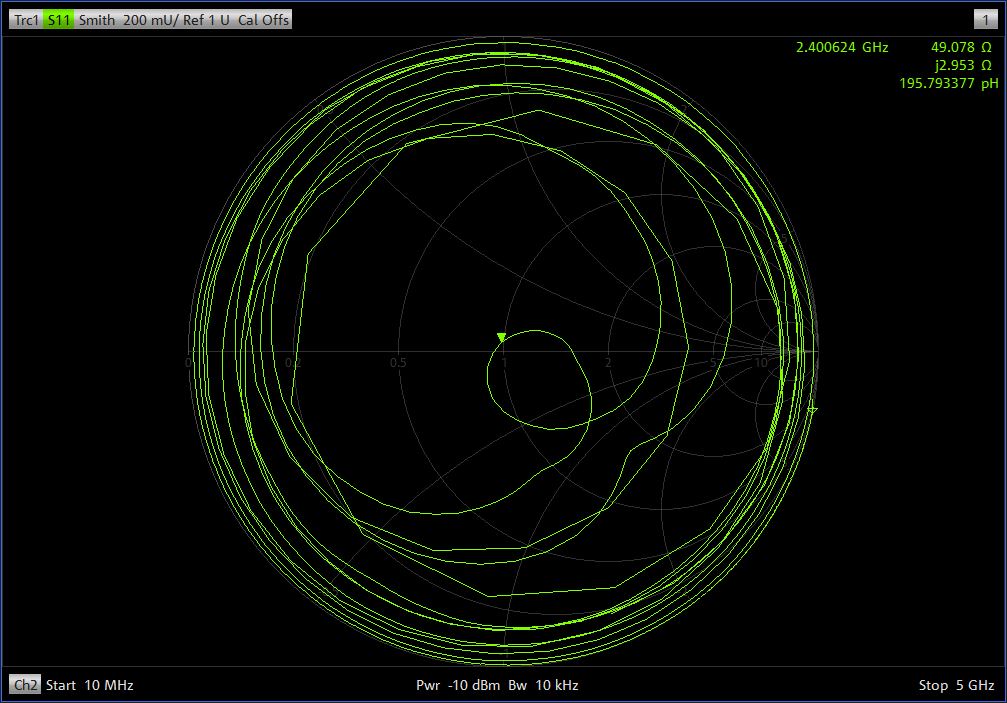
\includegraphics[width=0.8\textwidth]{src/figers/ex_3/Antenna_ss_turner_smith.png}
    \caption{Smith chart illustrating the impedance matching process using the slide-screw tuner at 2.4 GHz.}
    \label{fig:ss_tuner_smith}
\end{figure}

\begin{figure}[htpb]
    \centering
    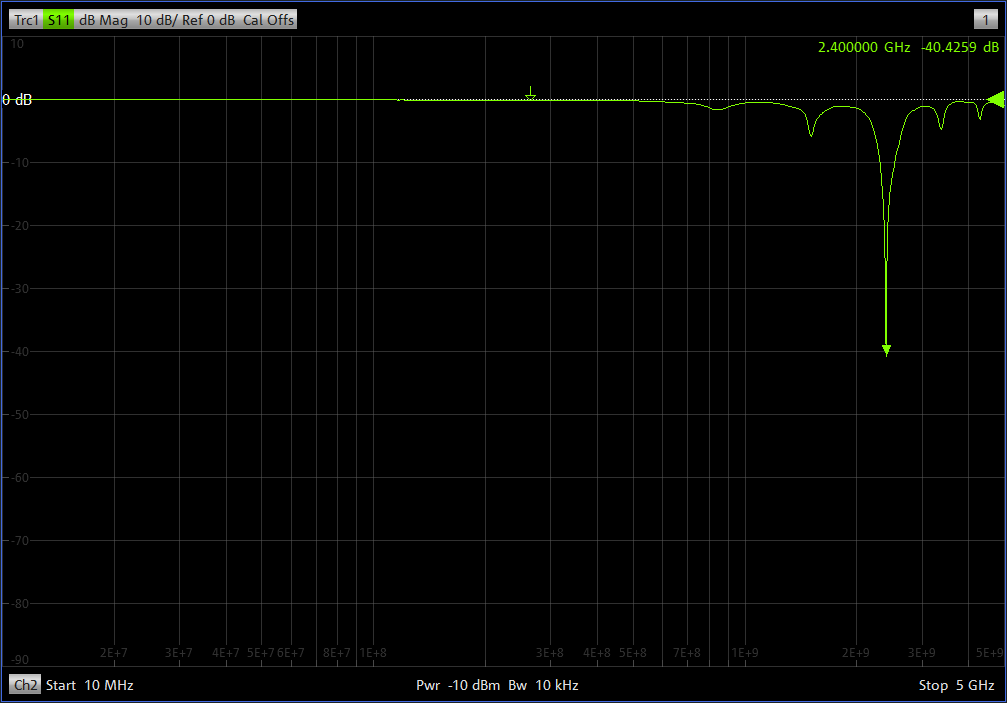
\includegraphics[width=0.8\textwidth]{src/figers/ex_3/Antenna_ss_turner_mag.png}
    \caption{Measured final reflection coefficient (logarithmic magnitude) of the antenna matched with the slide-screw tuner.}
    \label{fig:ss_tuner_mag}
\end{figure}
\FloatBarrier

\subsubsection{Short discussion of measurement results}

The unmatched antenna initially exhibited a high reflection coefficient of -5.27 dB at 2.4 GHz, which corresponds to a poor VSWR of 3.40. This means that a significant portion of the transmitted power was reflected due to the severe impedance mismatch.

By observing the Smith chart on the network analyser in real-time, the slide-screw tuner was adjusted. Lowering the slug ($Y$-direction) altered the magnitude of the reflection, while sliding it along the line ($X$-direction) rotated the phase. This effectively steered the impedance curve directly toward the matching point in the center of the Smith chart ($r=1$, $x=0$).

The final measurement yielded an excellent reflection coefficient of -40.4259 dB at 2.4 GHz, corresponding to a near-ideal VSWR of 1.02. The Smith chart confirms this, as the marker reading sits almost perfectly at the center (49.078 $\Omega$ + j2.953 $\Omega$), effectively cancelling out the reactive components of the unmatched antenna. This demonstrates that the mechanical slide-screw tuner successfully matched the antenna to the 50 $\Omega$ system, practically validating the theoretical matching principles without the need for fixed physical capacitors or transmission line segments.